\documentclass[9pt]{article}
\usepackage[a4paper,margin=14mm]{geometry}
\usepackage{graphicx}
\usepackage{booktabs}
\usepackage{longtable}
\usepackage{array}
\usepackage{hyperref}
\usepackage{caption}
\usepackage{float}
\usepackage{pdflscape}
\setlength{\parindent}{0pt}
\setlength{\parskip}{4pt}
\title{\textbf{Supplementary Material}\\[5pt]
\large Simple Pseudobulk Outperforms Topological and Quantum-Geometric Readouts\\
of Single-Nucleus Chromatin and Transcriptomes for Donor-Level Alzheimer's Classification:\\
A Rigorous Benchmark in a Powered Multiome Cohort}
\author{Sunjun Hwang and Dohyun Hwang}
\date{CKAIA 2026 --- Submission 10}
\hypersetup{
  pdftitle={Simple Pseudobulk Outperforms Topological and Quantum-Geometric Readouts of Single-Nucleus Chromatin and Transcriptomes for Donor-Level Alzheimer's Classification: A Rigorous Benchmark in a Powered Multiome Cohort --- Supplementary Material},
  pdfauthor={Sunjun Hwang and Dohyun Hwang}
}
\begin{document}
\maketitle

\section{Protocol, Representation Scope, and Uncertainty}
The primary binary contrast is late-AD versus non-AD. Before cell-class-specific filtering it contains 78 donors (21 late-AD, 57 non-AD). Four models were evaluated on identical donor sets and repeated $20\times5$ folds: covariates ($M_0$), covariates plus pseudobulk ($M_1$), covariates plus topology ($M_2$), and all features ($M_3$). The binary target was never residualized. Every fold-dependent downstream scaler, covariate encoding, and persistence-image range/bandwidth was fitted on training donors only. The LSI--Harmony embedding and COAST encoder were computed once on all donors without outcome labels and were not fold-wise retrained.

The 95\% intervals below are paired class-stratified percentile donor-bootstrap intervals based on the 20-repeat-averaged cross-fitted scores. The classifier and feature pipeline were not refitted inside bootstrap replicates; consequently, the intervals quantify donor-resampling uncertainty conditional on the fixed cross-fitted predictions. Repeat-level SDs are reported separately as descriptive split instability. No multiplicity adjustment was applied across 36 arms, and per-arm intervals are not interpreted as familywise discoveries.

\section{Arm-Level AUC and Incremental Comparisons}
\begin{figure}[H]
\centering
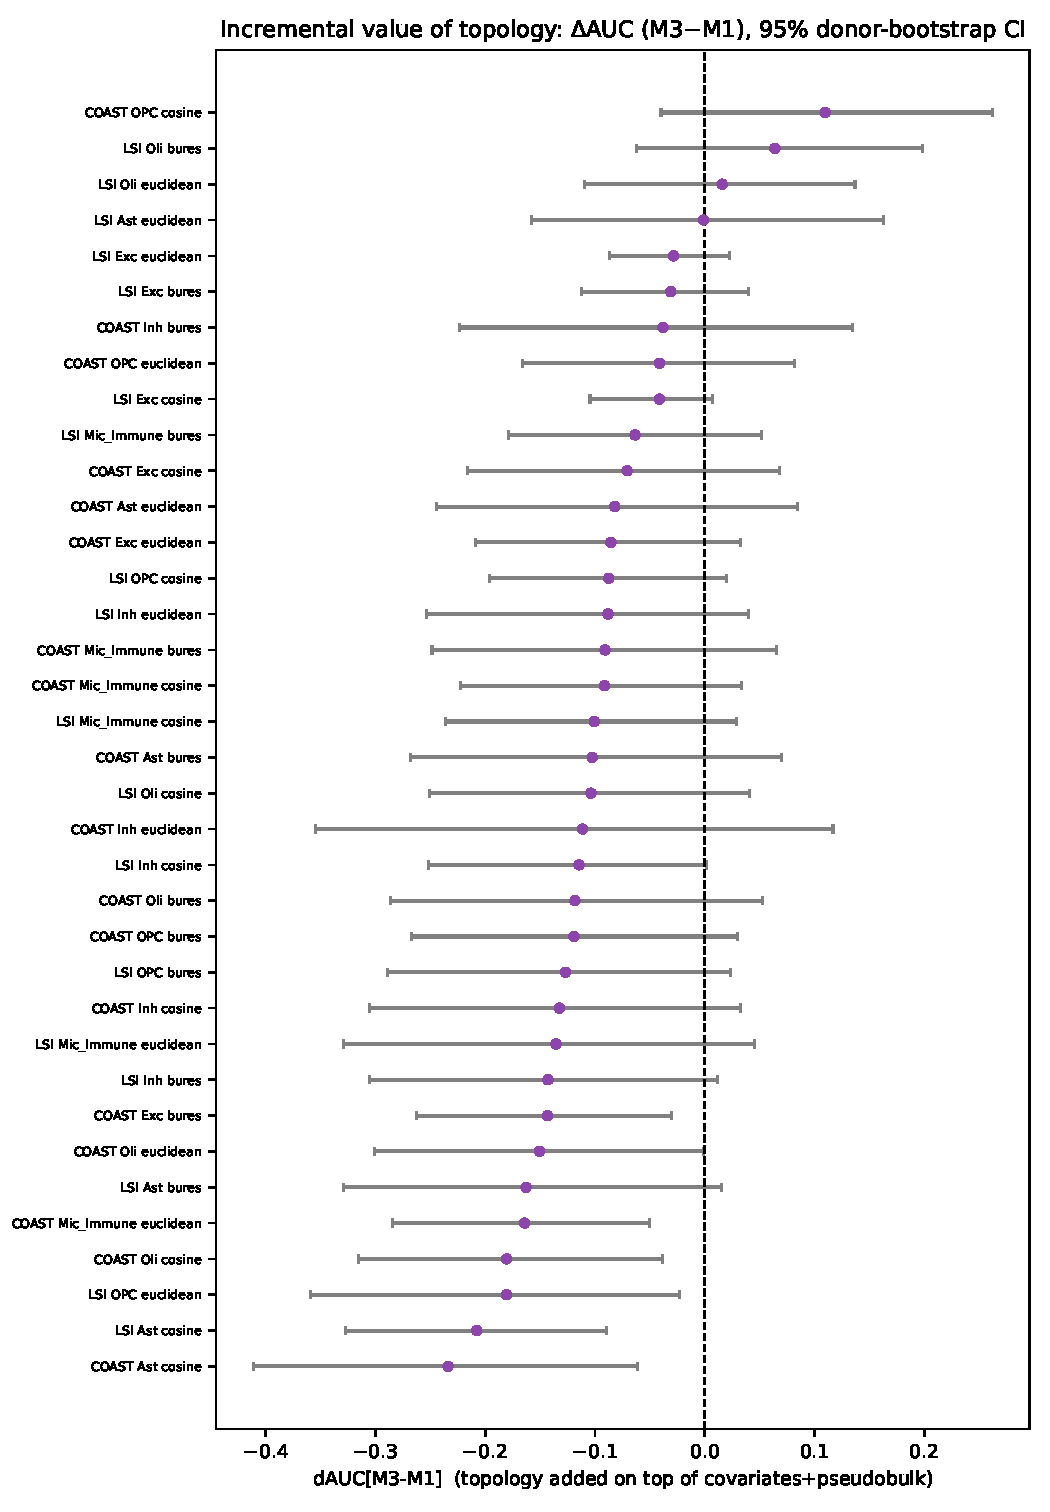
\includegraphics[width=0.58\textwidth]{confirmatory_analysis/figures/incremental_delta_auc_forest.pdf}
\caption{Paired $M_3-M_1$ AUC estimates. Intervals are unadjusted donor-resampling intervals conditional on fixed cross-fitted scores.}
\end{figure}
\clearpage

\begin{landscape}
\scriptsize
\begin{longtable}{lllrrrrrrr}
\caption{Arm-level AUC. Entries are estimate [95\% donor-resampling interval]. $n$ reports total donors (late-AD donors).}\\
\toprule
Latent & Cell & Metric & $n$ & $M_0$ & $M_1$ & $M_2$ & $M_3$ & $M_2-M_0$ & $M_3-M_1$ \\
\midrule
\endfirsthead
\toprule
Latent & Cell & Metric & $n$ & $M_0$ & $M_1$ & $M_2$ & $M_3$ & $M_2-M_0$ & $M_3-M_1$ \\
\midrule
\endhead
COAST & Exc & Bures & 71 (16) & 0.583 [0.420,0.742] & 0.766 [0.647,0.867] & 0.487 [0.340,0.634] & 0.623 [0.491,0.749] & -0.096 [-0.292,0.094] & -0.143 [-0.262,-0.031] \\
COAST & Exc & Cosine & 71 (16) & 0.583 [0.420,0.742] & 0.766 [0.647,0.867] & 0.482 [0.310,0.657] & 0.696 [0.535,0.841] & -0.101 [-0.305,0.088] & -0.071 [-0.216,0.068] \\
COAST & Exc & Euclidean & 71 (16) & 0.583 [0.420,0.742] & 0.766 [0.647,0.867] & 0.614 [0.469,0.753] & 0.681 [0.535,0.814] & 0.031 [-0.158,0.225] & -0.085 [-0.209,0.033] \\
COAST & Inh & Bures & 69 (14) & 0.496 [0.321,0.671] & 0.674 [0.530,0.808] & 0.689 [0.529,0.832] & 0.636 [0.477,0.788] & 0.193 [-0.047,0.430] & -0.038 [-0.223,0.135] \\
COAST & Inh & Cosine & 69 (14) & 0.496 [0.321,0.671] & 0.674 [0.530,0.808] & 0.391 [0.235,0.557] & 0.541 [0.392,0.691] & -0.105 [-0.317,0.110] & -0.132 [-0.305,0.032] \\
COAST & Inh & Euclidean & 69 (14) & 0.496 [0.321,0.671] & 0.674 [0.530,0.808] & 0.479 [0.296,0.660] & 0.562 [0.384,0.730] & -0.017 [-0.229,0.192] & -0.111 [-0.355,0.117] \\
COAST & Ast & Bures & 64 (16) & 0.547 [0.358,0.732] & 0.723 [0.577,0.849] & 0.583 [0.419,0.741] & 0.620 [0.462,0.770] & 0.037 [-0.147,0.238] & -0.102 [-0.268,0.070] \\
COAST & Ast & Cosine & 64 (16) & 0.547 [0.358,0.732] & 0.723 [0.577,0.849] & 0.488 [0.319,0.659] & 0.489 [0.324,0.658] & -0.059 [-0.268,0.145] & -0.234 [-0.411,-0.061] \\
COAST & Ast & Euclidean & 64 (16) & 0.547 [0.358,0.732] & 0.723 [0.577,0.849] & 0.615 [0.458,0.762] & 0.641 [0.495,0.776] & 0.068 [-0.145,0.283] & -0.082 [-0.245,0.085] \\
COAST & Oli & Bures & 74 (18) & 0.561 [0.384,0.733] & 0.676 [0.545,0.795] & 0.568 [0.404,0.723] & 0.558 [0.395,0.715] & 0.007 [-0.209,0.228] & -0.118 [-0.287,0.053] \\
COAST & Oli & Cosine & 74 (18) & 0.561 [0.384,0.733] & 0.676 [0.545,0.795] & 0.437 [0.301,0.581] & 0.496 [0.356,0.641] & -0.124 [-0.314,0.085] & -0.180 [-0.315,-0.039] \\
COAST & Oli & Euclidean & 74 (18) & 0.561 [0.384,0.733] & 0.676 [0.545,0.795] & 0.469 [0.303,0.639] & 0.526 [0.380,0.673] & -0.092 [-0.261,0.062] & -0.151 [-0.301,-0.001] \\
COAST & OPC & Bures & 57 (14) & 0.536 [0.352,0.714] & 0.550 [0.387,0.708] & 0.401 [0.249,0.556] & 0.431 [0.269,0.593] & -0.135 [-0.380,0.116] & -0.119 [-0.267,0.030] \\
COAST & OPC & Cosine & 57 (14) & 0.536 [0.352,0.714] & 0.550 [0.387,0.708] & 0.598 [0.434,0.751] & 0.660 [0.510,0.802] & 0.062 [-0.166,0.287] & 0.110 [-0.040,0.262] \\
COAST & OPC & Euclidean & 57 (14) & 0.536 [0.352,0.714] & 0.550 [0.387,0.708] & 0.572 [0.402,0.736] & 0.509 [0.347,0.673] & 0.036 [-0.233,0.294] & -0.041 [-0.166,0.081] \\
COAST & Micro & Bures & 59 (15) & 0.579 [0.394,0.758] & 0.712 [0.556,0.847] & 0.619 [0.450,0.783] & 0.621 [0.461,0.777] & 0.040 [-0.200,0.279] & -0.091 [-0.248,0.065] \\
COAST & Micro & Cosine & 59 (15) & 0.579 [0.394,0.758] & 0.712 [0.556,0.847] & 0.599 [0.420,0.765] & 0.620 [0.447,0.779] & 0.020 [-0.217,0.262] & -0.091 [-0.223,0.033] \\
COAST & Micro & Euclidean & 59 (15) & 0.579 [0.394,0.758] & 0.712 [0.556,0.847] & 0.533 [0.371,0.688] & 0.547 [0.379,0.708] & -0.046 [-0.261,0.168] & -0.164 [-0.285,-0.050] \\
LSI & Exc & Bures & 71 (16) & 0.583 [0.420,0.742] & 0.937 [0.858,0.991] & 0.595 [0.439,0.745] & 0.906 [0.818,0.970] & 0.012 [-0.226,0.250] & -0.031 [-0.112,0.040] \\
LSI & Exc & Cosine & 71 (16) & 0.583 [0.420,0.742] & 0.937 [0.858,0.991] & 0.617 [0.467,0.756] & 0.895 [0.795,0.972] & 0.033 [-0.188,0.255] & -0.041 [-0.105,0.007] \\
LSI & Exc & Euclidean & 71 (16) & 0.583 [0.420,0.742] & 0.937 [0.858,0.991] & 0.520 [0.375,0.659] & 0.908 [0.825,0.970] & -0.063 [-0.252,0.122] & -0.028 [-0.086,0.023] \\
LSI & Inh & Bures & 69 (14) & 0.496 [0.321,0.671] & 0.840 [0.714,0.940] & 0.465 [0.297,0.639] & 0.697 [0.535,0.842] & -0.032 [-0.264,0.201] & -0.143 [-0.305,0.012] \\
LSI & Inh & Cosine & 69 (14) & 0.496 [0.321,0.671] & 0.840 [0.714,0.940] & 0.510 [0.327,0.690] & 0.725 [0.565,0.870] & 0.013 [-0.219,0.245] & -0.114 [-0.252,0.001] \\
LSI & Inh & Euclidean & 69 (14) & 0.496 [0.321,0.671] & 0.840 [0.714,0.940] & 0.560 [0.392,0.727] & 0.751 [0.589,0.888] & 0.064 [-0.139,0.264] & -0.088 [-0.253,0.040] \\
LSI & Ast & Bures & 64 (16) & 0.547 [0.358,0.732] & 0.646 [0.495,0.788] & 0.444 [0.275,0.620] & 0.484 [0.336,0.637] & -0.103 [-0.290,0.077] & -0.163 [-0.329,0.016] \\
LSI & Ast & Cosine & 64 (16) & 0.547 [0.358,0.732] & 0.646 [0.495,0.788] & 0.468 [0.316,0.625] & 0.439 [0.296,0.589] & -0.079 [-0.279,0.115] & -0.208 [-0.327,-0.090] \\
LSI & Ast & Euclidean & 64 (16) & 0.547 [0.358,0.732] & 0.646 [0.495,0.788] & 0.479 [0.303,0.658] & 0.645 [0.495,0.785] & -0.068 [-0.258,0.118] & -0.001 [-0.158,0.163] \\
LSI & Oli & Bures & 74 (18) & 0.561 [0.384,0.733] & 0.708 [0.577,0.830] & 0.695 [0.536,0.835] & 0.772 [0.654,0.873] & 0.134 [-0.050,0.315] & 0.064 [-0.062,0.198] \\
LSI & Oli & Cosine & 74 (18) & 0.561 [0.384,0.733] & 0.708 [0.577,0.830] & 0.577 [0.427,0.726] & 0.605 [0.455,0.745] & 0.015 [-0.209,0.243] & -0.104 [-0.251,0.041] \\
LSI & Oli & Euclidean & 74 (18) & 0.561 [0.384,0.733] & 0.708 [0.577,0.830] & 0.679 [0.524,0.819] & 0.724 [0.597,0.842] & 0.118 [-0.105,0.332] & 0.016 [-0.109,0.137] \\
LSI & OPC & Bures & 57 (14) & 0.536 [0.352,0.714] & 0.809 [0.678,0.914] & 0.604 [0.419,0.779] & 0.682 [0.503,0.849] & 0.067 [-0.158,0.284] & -0.127 [-0.289,0.023] \\
LSI & OPC & Cosine & 57 (14) & 0.536 [0.352,0.714] & 0.809 [0.678,0.914] & 0.646 [0.463,0.816] & 0.721 [0.547,0.874] & 0.110 [-0.123,0.342] & -0.087 [-0.196,0.020] \\
LSI & OPC & Euclidean & 57 (14) & 0.536 [0.352,0.714] & 0.809 [0.678,0.914] & 0.533 [0.344,0.718] & 0.628 [0.447,0.801] & -0.003 [-0.254,0.243] & -0.181 [-0.359,-0.023] \\
LSI & Micro & Bures & 59 (15) & 0.579 [0.394,0.758] & 0.732 [0.589,0.859] & 0.587 [0.418,0.745] & 0.669 [0.517,0.809] & 0.008 [-0.158,0.179] & -0.063 [-0.179,0.052] \\
LSI & Micro & Cosine & 59 (15) & 0.579 [0.394,0.758] & 0.732 [0.589,0.859] & 0.631 [0.465,0.782] & 0.632 [0.464,0.786] & 0.052 [-0.176,0.276] & -0.101 [-0.236,0.029] \\
LSI & Micro & Euclidean & 59 (15) & 0.579 [0.394,0.758] & 0.732 [0.589,0.859] & 0.594 [0.405,0.776] & 0.597 [0.417,0.770] & 0.015 [-0.145,0.173] & -0.136 [-0.329,0.045] \\
\bottomrule
\end{longtable}
\footnotesize
Across the 36 arms, $M_2-M_0$ averaged $\Delta$AUC 0.000; 21 point estimates were positive, but none of the intervals excluded zero in either direction. For $M_3-M_1$, 33 point estimates were negative. Seven upper bounds were below zero before multiplicity correction; this count is descriptive only.
\end{landscape}

\section{Balanced Accuracy}
\begin{figure}[H]
\centering
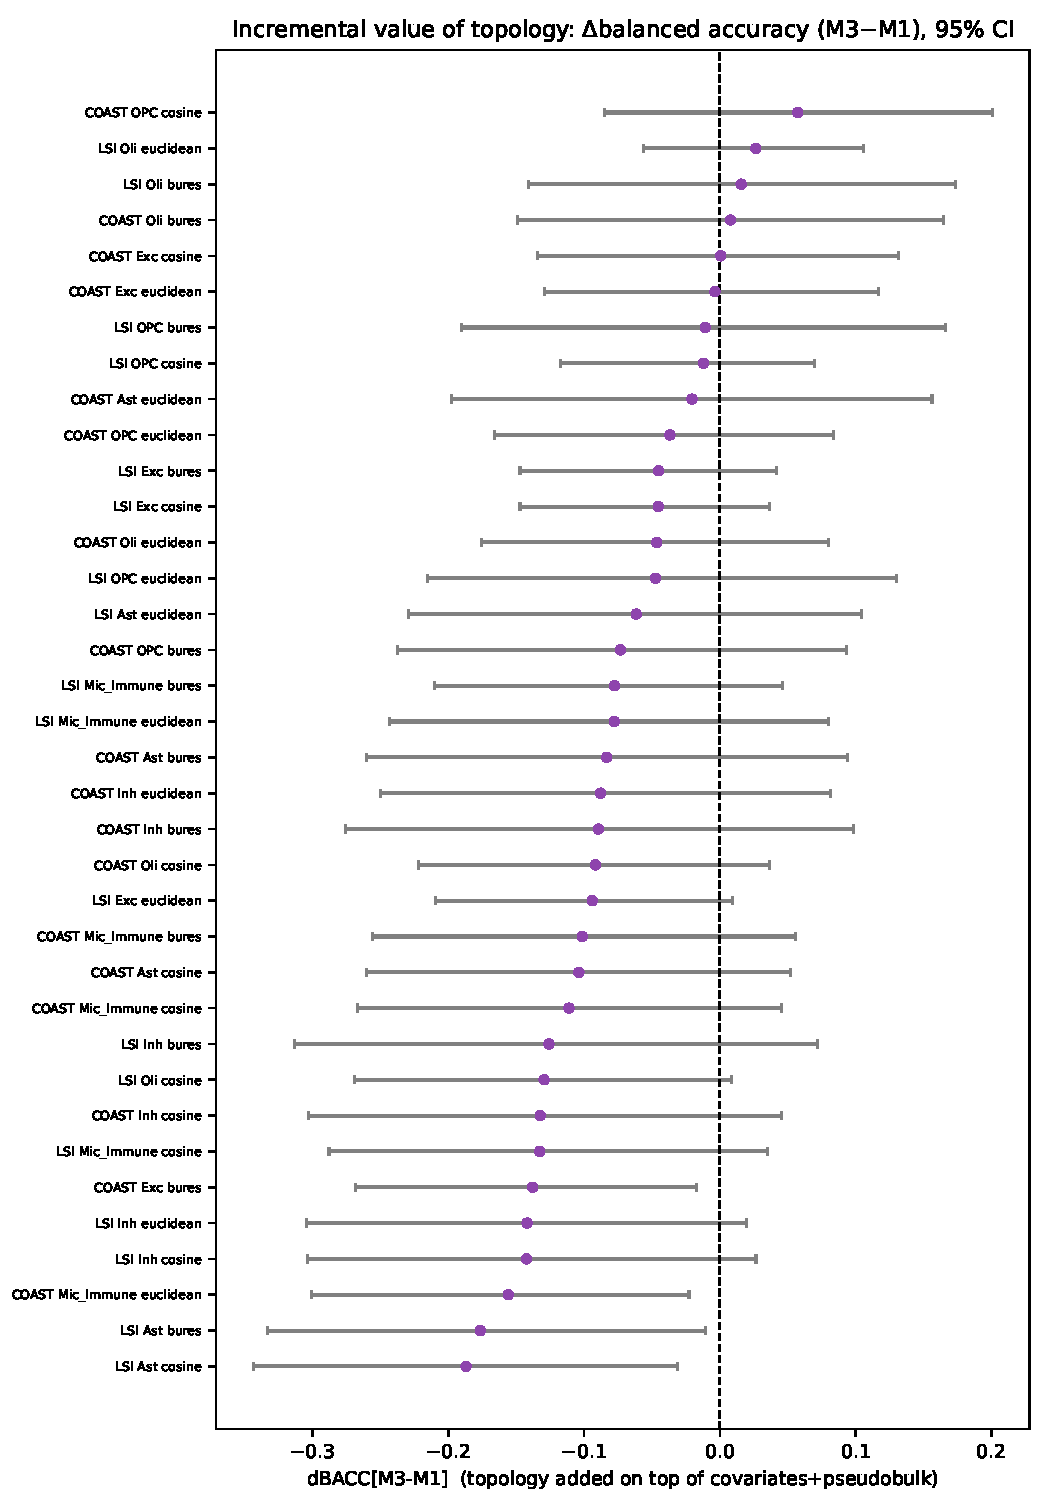
\includegraphics[width=0.58\textwidth]{confirmatory_analysis/figures/incremental_delta_balanced_accuracy_forest.pdf}
\caption{Paired $M_3-M_1$ balanced-accuracy estimates.}
\end{figure}
\clearpage

\begin{landscape}
\scriptsize
\begin{longtable}{lllrrrrrrr}
\caption{Arm-level balanced accuracy. Entries are estimate [95\% donor-resampling interval].}\\
\toprule
Latent & Cell & Metric & $n$ & $M_0$ & $M_1$ & $M_2$ & $M_3$ & $M_2-M_0$ & $M_3-M_1$ \\
\midrule
\endfirsthead
\toprule
Latent & Cell & Metric & $n$ & $M_0$ & $M_1$ & $M_2$ & $M_3$ & $M_2-M_0$ & $M_3-M_1$ \\
\midrule
\endhead
COAST & Exc & Bures & 71 (16) & 0.631 [0.493,0.761] & 0.645 [0.511,0.775] & 0.449 [0.345,0.565] & 0.507 [0.395,0.633] & -0.181 [-0.344,-0.012] & -0.138 [-0.268,-0.017] \\
COAST & Exc & Cosine & 71 (16) & 0.631 [0.493,0.761] & 0.645 [0.511,0.775] & 0.547 [0.426,0.677] & 0.646 [0.520,0.776] & -0.084 [-0.228,0.053] & 0.001 [-0.134,0.131] \\
COAST & Exc & Euclidean & 71 (16) & 0.631 [0.493,0.761] & 0.645 [0.511,0.775] & 0.497 [0.386,0.623] & 0.641 [0.507,0.775] & -0.133 [-0.290,0.032] & -0.004 [-0.129,0.117] \\
COAST & Inh & Bures & 69 (14) & 0.603 [0.460,0.738] & 0.604 [0.461,0.748] & 0.605 [0.480,0.740] & 0.515 [0.390,0.651] & 0.002 [-0.186,0.200] & -0.090 [-0.276,0.099] \\
COAST & Inh & Cosine & 69 (14) & 0.603 [0.460,0.738] & 0.604 [0.461,0.748] & 0.454 [0.355,0.570] & 0.472 [0.373,0.588] & -0.149 [-0.321,0.039] & -0.132 [-0.303,0.045] \\
COAST & Inh & Euclidean & 69 (14) & 0.603 [0.460,0.738] & 0.604 [0.461,0.748] & 0.533 [0.399,0.676] & 0.516 [0.408,0.642] & -0.070 [-0.240,0.101] & -0.088 [-0.250,0.081] \\
COAST & Ast & Bures & 64 (16) & 0.541 [0.406,0.688] & 0.594 [0.469,0.729] & 0.583 [0.438,0.719] & 0.510 [0.385,0.646] & 0.041 [-0.125,0.208] & -0.083 [-0.260,0.094] \\
COAST & Ast & Cosine & 64 (16) & 0.541 [0.406,0.688] & 0.594 [0.469,0.729] & 0.532 [0.396,0.667] & 0.490 [0.375,0.615] & -0.009 [-0.156,0.125] & -0.104 [-0.260,0.052] \\
COAST & Ast & Euclidean & 64 (16) & 0.541 [0.406,0.688] & 0.594 [0.469,0.729] & 0.521 [0.385,0.656] & 0.573 [0.438,0.708] & -0.020 [-0.188,0.146] & -0.021 [-0.198,0.156] \\
COAST & Oli & Bures & 74 (18) & 0.608 [0.479,0.736] & 0.550 [0.424,0.681] & 0.532 [0.413,0.654] & 0.558 [0.440,0.680] & -0.077 [-0.259,0.105] & 0.008 [-0.149,0.165] \\
COAST & Oli & Cosine & 74 (18) & 0.608 [0.479,0.736] & 0.550 [0.424,0.681] & 0.404 [0.304,0.515] & 0.459 [0.350,0.578] & -0.204 [-0.360,-0.041] & -0.092 [-0.222,0.037] \\
COAST & Oli & Euclidean & 74 (18) & 0.608 [0.479,0.736] & 0.550 [0.424,0.681] & 0.497 [0.377,0.625] & 0.504 [0.394,0.626] & -0.112 [-0.249,0.015] & -0.046 [-0.176,0.080] \\
COAST & OPC & Bures & 57 (14) & 0.529 [0.375,0.683] & 0.505 [0.363,0.649] & 0.421 [0.314,0.540] & 0.432 [0.326,0.551] & -0.108 [-0.298,0.081] & -0.073 [-0.238,0.093] \\
COAST & OPC & Cosine & 57 (14) & 0.529 [0.375,0.683] & 0.505 [0.363,0.649] & 0.503 [0.373,0.645] & 0.563 [0.421,0.705] & -0.026 [-0.227,0.178] & 0.057 [-0.085,0.201] \\
COAST & OPC & Euclidean & 57 (14) & 0.529 [0.375,0.683] & 0.505 [0.363,0.649] & 0.517 [0.375,0.659] & 0.469 [0.338,0.610] & -0.012 [-0.226,0.201] & -0.037 [-0.166,0.084] \\
COAST & Micro & Bures & 59 (15) & 0.551 [0.405,0.697] & 0.665 [0.519,0.798] & 0.575 [0.430,0.720] & 0.563 [0.428,0.709] & 0.024 [-0.209,0.258] & -0.101 [-0.256,0.056] \\
COAST & Micro & Cosine & 59 (15) & 0.551 [0.405,0.697] & 0.665 [0.519,0.798] & 0.587 [0.452,0.731] & 0.553 [0.420,0.687] & 0.036 [-0.166,0.238] & -0.111 [-0.267,0.045] \\
COAST & Micro & Euclidean & 59 (15) & 0.551 [0.405,0.697] & 0.665 [0.519,0.798] & 0.509 [0.386,0.642] & 0.509 [0.373,0.652] & -0.042 [-0.211,0.125] & -0.156 [-0.301,-0.023] \\
LSI & Exc & Bures & 71 (16) & 0.631 [0.493,0.761] & 0.844 [0.731,0.941] & 0.539 [0.416,0.673] & 0.798 [0.673,0.910] & -0.092 [-0.276,0.096] & -0.045 [-0.147,0.041] \\
LSI & Exc & Cosine & 71 (16) & 0.631 [0.493,0.761] & 0.844 [0.731,0.941] & 0.547 [0.426,0.677] & 0.798 [0.673,0.910] & -0.083 [-0.258,0.104] & -0.045 [-0.147,0.036] \\
LSI & Exc & Euclidean & 71 (16) & 0.631 [0.493,0.761] & 0.844 [0.731,0.941] & 0.444 [0.355,0.547] & 0.750 [0.620,0.874] & -0.187 [-0.330,-0.043] & -0.094 [-0.210,0.009] \\
LSI & Inh & Bures & 69 (14) & 0.603 [0.460,0.738] & 0.758 [0.623,0.882] & 0.489 [0.399,0.597] & 0.632 [0.498,0.768] & -0.113 [-0.284,0.074] & -0.126 [-0.313,0.072] \\
LSI & Inh & Cosine & 69 (14) & 0.603 [0.460,0.738] & 0.758 [0.623,0.882] & 0.498 [0.381,0.624] & 0.616 [0.480,0.758] & -0.105 [-0.276,0.083] & -0.142 [-0.304,0.027] \\
LSI & Inh & Euclidean & 69 (14) & 0.603 [0.460,0.738] & 0.758 [0.623,0.882] & 0.515 [0.390,0.650] & 0.616 [0.480,0.758] & -0.088 [-0.240,0.056] & -0.142 [-0.305,0.019] \\
LSI & Ast & Bures & 64 (16) & 0.541 [0.406,0.688] & 0.614 [0.469,0.750] & 0.490 [0.375,0.615] & 0.438 [0.312,0.573] & -0.052 [-0.208,0.104] & -0.176 [-0.333,-0.010] \\
LSI & Ast & Cosine & 64 (16) & 0.541 [0.406,0.688] & 0.614 [0.469,0.750] & 0.437 [0.323,0.552] & 0.427 [0.302,0.562] & -0.104 [-0.271,0.062] & -0.187 [-0.344,-0.031] \\
LSI & Ast & Euclidean & 64 (16) & 0.541 [0.406,0.688] & 0.614 [0.469,0.750] & 0.531 [0.406,0.667] & 0.552 [0.417,0.688] & -0.010 [-0.167,0.135] & -0.062 [-0.229,0.104] \\
LSI & Oli & Bures & 74 (18) & 0.608 [0.479,0.736] & 0.634 [0.505,0.763] & 0.679 [0.559,0.799] & 0.650 [0.531,0.771] & 0.070 [-0.085,0.225] & 0.016 [-0.141,0.174] \\
LSI & Oli & Cosine & 74 (18) & 0.608 [0.479,0.736] & 0.634 [0.505,0.763] & 0.550 [0.439,0.669] & 0.505 [0.393,0.625] & -0.058 [-0.225,0.116] & -0.129 [-0.269,0.009] \\
LSI & Oli & Euclidean & 74 (18) & 0.608 [0.479,0.736] & 0.634 [0.505,0.763] & 0.625 [0.503,0.753] & 0.661 [0.533,0.789] & 0.017 [-0.161,0.198] & 0.026 [-0.057,0.106] \\
LSI & OPC & Bures & 57 (14) & 0.529 [0.375,0.683] & 0.680 [0.538,0.823] & 0.575 [0.444,0.716] & 0.670 [0.527,0.811] & 0.046 [-0.130,0.209] & -0.011 [-0.190,0.166] \\
LSI & OPC & Cosine & 57 (14) & 0.529 [0.375,0.683] & 0.680 [0.538,0.823] & 0.657 [0.514,0.799] & 0.668 [0.527,0.811] & 0.128 [-0.072,0.328] & -0.012 [-0.117,0.070] \\
LSI & OPC & Euclidean & 57 (14) & 0.529 [0.375,0.683] & 0.680 [0.538,0.823] & 0.586 [0.455,0.728] & 0.633 [0.492,0.776] & 0.057 [-0.133,0.247] & -0.047 [-0.215,0.130] \\
LSI & Micro & Bures & 59 (15) & 0.551 [0.405,0.697] & 0.664 [0.518,0.797] & 0.519 [0.397,0.653] & 0.586 [0.452,0.721] & -0.032 [-0.199,0.136] & -0.078 [-0.210,0.046] \\
LSI & Micro & Cosine & 59 (15) & 0.551 [0.405,0.697] & 0.664 [0.518,0.797] & 0.554 [0.431,0.677] & 0.531 [0.408,0.664] & 0.002 [-0.187,0.192] & -0.133 [-0.288,0.035] \\
LSI & Micro & Euclidean & 59 (15) & 0.551 [0.405,0.697] & 0.664 [0.518,0.797] & 0.620 [0.476,0.764] & 0.586 [0.452,0.730] & 0.069 [-0.098,0.236] & -0.078 [-0.243,0.080] \\
\bottomrule
\end{longtable}
\footnotesize
Mean $M_3-M_1$ balanced-accuracy difference was $-0.074$. Five point estimates were positive; no lower interval bound exceeded zero. Four upper bounds were below zero before multiplicity correction.
\end{landscape}

\begin{landscape}
\section{Repeat-Level Split Instability}
The following repeat-level summaries are descriptive only because the 20 repeated-CV estimates share donors and overlapping training sets.
\footnotesize
\begin{longtable}{lllrrr}
\caption{Repeat-level paired differences over 20 repeats.}\\
\toprule
Latent & Cell & Metric & $\Delta$AUC mean $\pm$ SD & $\Delta$AUC range & $\Delta$BAcc mean $\pm$ SD \\
\midrule
\endfirsthead
\toprule
Latent & Cell & Metric & $\Delta$AUC mean $\pm$ SD & $\Delta$AUC range & $\Delta$BAcc mean $\pm$ SD \\
\midrule
\endhead
COAST & Exc & Bures & -0.148 $\pm$ 0.061 & [-0.244,-0.030] & -0.141 $\pm$ 0.066 \\
COAST & Exc & Cosine & -0.138 $\pm$ 0.069 & [-0.311,-0.019] & -0.027 $\pm$ 0.063 \\
COAST & Exc & Euclidean & -0.100 $\pm$ 0.056 & [-0.214,0.005] & -0.045 $\pm$ 0.060 \\
COAST & Inh & Bures & -0.083 $\pm$ 0.060 & [-0.205,0.038] & -0.041 $\pm$ 0.062 \\
COAST & Inh & Cosine & -0.140 $\pm$ 0.074 & [-0.244,0.066] & -0.099 $\pm$ 0.069 \\
COAST & Inh & Euclidean & -0.106 $\pm$ 0.055 & [-0.197,-0.009] & -0.073 $\pm$ 0.090 \\
COAST & Ast & Bures & -0.090 $\pm$ 0.051 & [-0.195,-0.003] & -0.031 $\pm$ 0.059 \\
COAST & Ast & Cosine & -0.210 $\pm$ 0.039 & [-0.276,-0.145] & -0.087 $\pm$ 0.062 \\
COAST & Ast & Euclidean & -0.057 $\pm$ 0.045 & [-0.121,0.029] & -0.027 $\pm$ 0.071 \\
COAST & Oli & Bures & -0.158 $\pm$ 0.067 & [-0.318,-0.036] & -0.026 $\pm$ 0.065 \\
COAST & Oli & Cosine & -0.177 $\pm$ 0.061 & [-0.281,-0.061] & -0.099 $\pm$ 0.052 \\
COAST & Oli & Euclidean & -0.151 $\pm$ 0.040 & [-0.209,-0.077] & -0.054 $\pm$ 0.042 \\
COAST & OPC & Bures & -0.166 $\pm$ 0.076 & [-0.311,-0.033] & -0.056 $\pm$ 0.059 \\
COAST & OPC & Cosine & 0.085 $\pm$ 0.055 & [-0.007,0.190] & 0.067 $\pm$ 0.066 \\
COAST & OPC & Euclidean & -0.037 $\pm$ 0.060 & [-0.121,0.085] & -0.008 $\pm$ 0.054 \\
COAST & Micro & Bures & -0.139 $\pm$ 0.089 & [-0.334,-0.012] & -0.090 $\pm$ 0.092 \\
COAST & Micro & Cosine & -0.086 $\pm$ 0.055 & [-0.185,0.021] & -0.092 $\pm$ 0.050 \\
COAST & Micro & Euclidean & -0.139 $\pm$ 0.048 & [-0.223,-0.042] & -0.141 $\pm$ 0.066 \\
LSI & Exc & Bures & -0.128 $\pm$ 0.049 & [-0.223,-0.024] & -0.070 $\pm$ 0.046 \\
LSI & Exc & Cosine & -0.057 $\pm$ 0.032 & [-0.125,0.003] & -0.075 $\pm$ 0.045 \\
LSI & Exc & Euclidean & -0.084 $\pm$ 0.048 & [-0.221,-0.002] & -0.080 $\pm$ 0.056 \\
LSI & Inh & Bures & -0.221 $\pm$ 0.070 & [-0.362,-0.078] & -0.112 $\pm$ 0.055 \\
LSI & Inh & Cosine & -0.121 $\pm$ 0.048 & [-0.196,-0.033] & -0.115 $\pm$ 0.058 \\
LSI & Inh & Euclidean & -0.121 $\pm$ 0.062 & [-0.255,-0.010] & -0.103 $\pm$ 0.070 \\
LSI & Ast & Bures & -0.164 $\pm$ 0.071 & [-0.290,-0.053] & -0.106 $\pm$ 0.066 \\
LSI & Ast & Cosine & -0.162 $\pm$ 0.049 & [-0.273,-0.058] & -0.136 $\pm$ 0.058 \\
LSI & Ast & Euclidean & -0.016 $\pm$ 0.053 & [-0.114,0.084] & 0.001 $\pm$ 0.054 \\
LSI & Oli & Bures & -0.010 $\pm$ 0.049 & [-0.109,0.076] & 0.001 $\pm$ 0.065 \\
LSI & Oli & Cosine & -0.108 $\pm$ 0.043 & [-0.182,-0.029] & -0.102 $\pm$ 0.049 \\
LSI & Oli & Euclidean & -0.045 $\pm$ 0.066 & [-0.149,0.078] & -0.033 $\pm$ 0.075 \\
LSI & OPC & Bures & -0.118 $\pm$ 0.043 & [-0.199,-0.057] & -0.035 $\pm$ 0.057 \\
LSI & OPC & Cosine & -0.069 $\pm$ 0.044 & [-0.161,-0.010] & -0.044 $\pm$ 0.057 \\
LSI & OPC & Euclidean & -0.165 $\pm$ 0.062 & [-0.292,-0.053] & -0.085 $\pm$ 0.073 \\
LSI & Micro & Bures & -0.093 $\pm$ 0.053 & [-0.191,0.058] & -0.077 $\pm$ 0.060 \\
LSI & Micro & Cosine & -0.145 $\pm$ 0.036 & [-0.227,-0.096] & -0.113 $\pm$ 0.059 \\
LSI & Micro & Euclidean & -0.109 $\pm$ 0.060 & [-0.248,0.011] & -0.092 $\pm$ 0.069 \\
\bottomrule
\end{longtable}
\end{landscape}

\section{Matched-Nucleus Standalone Sensitivity}
COAST pseudobulk and COAST--Bures H1 features used identical nucleus IDs. Three deterministic nucleus-sampling seeds were averaged; seed-specific performance was not retained and no seed-level SD is claimed. The comparison is standalone and does not estimate matched-nucleus $M_3-M_1$.

\begin{figure}[ht]
\centering
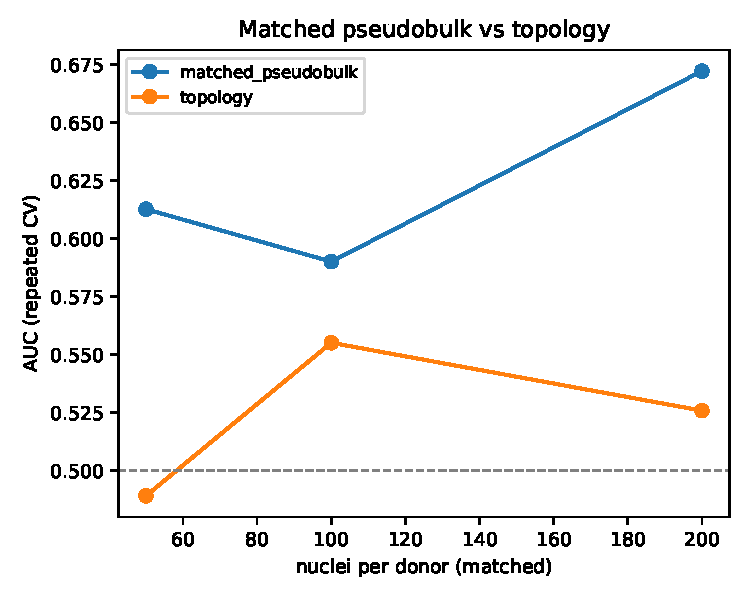
\includegraphics[width=0.66\textwidth]{confirmatory_analysis/figures/auc_vs_subsample_size.pdf}
\caption{Mean AUC across cell classes versus matched nucleus count. Non-monotonicity is visible and should be considered when interpreting the 200-nucleus result.}
\end{figure}

\begin{table}[ht]
\centering
\scriptsize
\caption{Matched performance by cell class and nucleus count.}
\begin{tabular}{lrrrrrrr}
\toprule
Cell & Nuclei & PB AUC & H1 AUC & $\Delta$AUC & PB BAcc & H1 BAcc & $\Delta$BAcc \\
\midrule
Exc & 50 & 0.810 & 0.426 & +0.384 & 0.684 & 0.460 & +0.224 \\
Exc & 100 & 0.632 & 0.547 & +0.085 & 0.554 & 0.517 & +0.036 \\
Exc & 200 & 0.596 & 0.466 & +0.130 & 0.507 & 0.458 & +0.048 \\
Inh & 50 & 0.571 & 0.473 & +0.099 & 0.493 & 0.468 & +0.025 \\
Inh & 100 & 0.611 & 0.679 & -0.068 & 0.543 & 0.613 & -0.070 \\
Inh & 200 & 0.764 & 0.622 & +0.142 & 0.661 & 0.543 & +0.118 \\
Ast & 50 & 0.565 & 0.490 & +0.074 & 0.528 & 0.493 & +0.034 \\
Ast & 100 & 0.540 & 0.566 & -0.026 & 0.542 & 0.594 & -0.052 \\
Ast & 200 & 0.732 & 0.554 & +0.178 & 0.696 & 0.576 & +0.120 \\
Oli & 50 & 0.560 & 0.387 & +0.173 & 0.530 & 0.439 & +0.091 \\
Oli & 100 & 0.647 & 0.528 & +0.119 & 0.590 & 0.506 & +0.084 \\
Oli & 200 & 0.678 & 0.599 & +0.079 & 0.601 & 0.584 & +0.017 \\
OPC & 50 & 0.520 & 0.626 & -0.106 & 0.496 & 0.597 & -0.101 \\
OPC & 100 & 0.547 & 0.444 & +0.103 & 0.541 & 0.434 & +0.107 \\
OPC & 200 & 0.625 & 0.507 & +0.118 & 0.601 & 0.476 & +0.125 \\
Micro & 50 & 0.650 & 0.534 & +0.117 & 0.608 & 0.486 & +0.122 \\
Micro & 100 & 0.564 & 0.568 & -0.004 & 0.572 & 0.532 & +0.040 \\
Micro & 200 & 0.638 & 0.407 & +0.230 & 0.574 & 0.436 & +0.138 \\
\bottomrule
\end{tabular}
\end{table}

\section{Idealized Simulations}
Each condition used 60 donors (15 cases), 120 nuclei per donor, and 30 generated datasets. Values are mean $\pm$ SD across datasets. The simulations are implementation detectability controls, not biological generative models or a complete power study.

\begin{figure}[H]
\centering
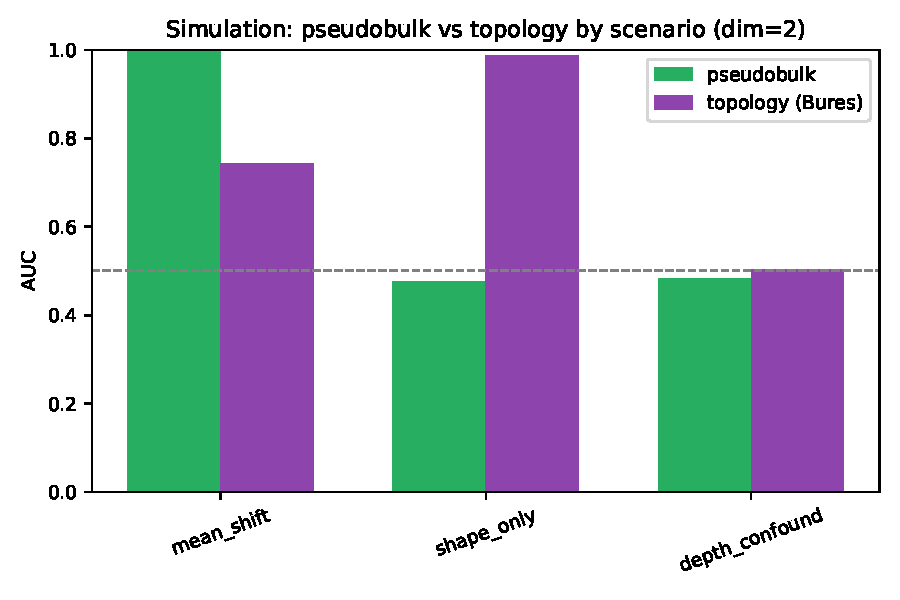
\includegraphics[width=0.67\textwidth]{confirmatory_analysis/figures/simulation_auc_by_scenario.pdf}
\caption{Two-dimensional simulation results.}
\end{figure}

\begin{figure}[H]
\centering
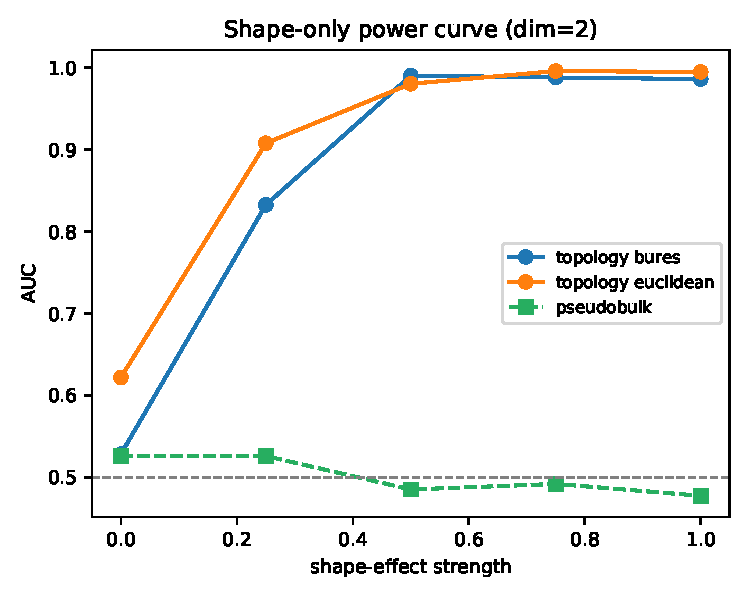
\includegraphics[width=0.67\textwidth]{confirmatory_analysis/figures/simulation_power_curve.pdf}
\caption{Two-dimensional shape-only effect sweep. The main 32-dimensional condition was evaluated at one effect setting and should not be generalized as a full dimensionality power curve.}
\end{figure}

\begin{table}[H]
\centering
\scriptsize
\caption{Simulation AUC mean $\pm$ SD across 30 datasets.}
\begin{tabular}{lrlrrr}
\toprule
Scenario & Dim. & Metric & Pseudobulk & H1 topology & PB+H1 \\
\midrule
null & 2 & Bures & 0.500 $\pm$ 0.113 & 0.503 $\pm$ 0.072 & 0.500 $\pm$ 0.070 \\
null & 32 & Bures & 0.483 $\pm$ 0.086 & 0.507 $\pm$ 0.096 & 0.493 $\pm$ 0.090 \\
mean shift & 2 & Bures & 1.000 $\pm$ 0.000 & 0.743 $\pm$ 0.075 & 0.788 $\pm$ 0.077 \\
mean shift & 32 & Bures & 0.996 $\pm$ 0.005 & 0.507 $\pm$ 0.094 & 0.809 $\pm$ 0.056 \\
shape only & 2 & Bures & 0.477 $\pm$ 0.126 & 0.986 $\pm$ 0.018 & 0.986 $\pm$ 0.018 \\
shape only & 32 & Bures & 0.514 $\pm$ 0.097 & 0.484 $\pm$ 0.081 & 0.499 $\pm$ 0.087 \\
depth confound & 2 & Bures & 0.484 $\pm$ 0.092 & 0.503 $\pm$ 0.068 & 0.497 $\pm$ 0.068 \\
depth confound & 32 & Bures & 0.489 $\pm$ 0.083 & 0.493 $\pm$ 0.112 & 0.494 $\pm$ 0.097 \\
shape only & 2 & Euclidean & 0.477 $\pm$ 0.126 & 0.995 $\pm$ 0.009 & 0.995 $\pm$ 0.009 \\
shape only & 32 & Euclidean & 0.514 $\pm$ 0.097 & 0.540 $\pm$ 0.104 & 0.546 $\pm$ 0.090 \\
\bottomrule
\end{tabular}
\end{table}

\section{Interpretive Qualifications}
The empirical analysis does not include a dimension-matched random-feature control, fold-wise feature selection or PCA, an equivalence test, full-pipeline bootstrap refitting, fold-wise COAST retraining, or an independent AD replication cohort. Adding 148 H1 features to approximately 46--59 training donors per cell-class fold can itself raise estimation variance. The negative $M_3-M_1$ results therefore describe the operational performance of the full readout, not proof that the feature family contains no weak signal. The 32-dimensional simulation further prevents distinguishing a biological absence of non-mean signal from pipeline power loss in nuisance-rich representations.

\section{Reproducibility and Data Access}
The accompanying \texttt{confirmatory\_analysis/} directory contains source code, frozen configuration, fold assignments, cross-fitted predictions, sampled nucleus IDs, machine-readable tables, and figures. Large cohort inputs are not redistributed. \texttt{INPUTS\_NOTE.txt} and \texttt{DATA\_PROVENANCE.md} record expected input names and the distinction between processed outputs and controlled raw data/metadata. The source project's applicable access terms must be followed.

\end{document}
